% simple.tex -- a very simple thesis document for demonstrating
%   dalthesis.cls class file
\documentclass[12pt]{dalthesis}
\usepackage{longtable}
\usepackage{multicol}
\usepackage{multirow}
\usepackage{subfigure}
\usepackage{graphicx}
\usepackage[toc,page]{appendix}
\usepackage{listings}
\usepackage{pgfplots}
\usepackage[backref]{hyperref}


\makeatletter
\def\dal@chapter[#1]#2{%
\ifnum \c@secnumdepth >\m@ne\refstepcounter{chapter}%
\typeout{\@chapapp\space\thechapter.}%
\addcontentsline{toc}{chapter}%
{\protect\numberline{\@chapapp\space\thechapter}#1}%
\else\addcontentsline{toc}{chapter}{#1}%
\fi\chaptermark{#1}%
\addtocontents{lof}{\protect\addvspace{10\p@}}%
\addtocontents{lot}{\protect\addvspace{10\p@}}%
\if@twocolumn\@topnewpage[\@makechapterhead{#2}]%
\else\@makechapterhead{#2}%
\@afterheading\fi%
\ifdal@in@preface\else\afterpage{\dal@add@textheight{\footskip}}\fi%
}
\makeatother


\begin{document}



\title{Analysis of Direct Bank Marketing Classification with Decision Tree}
\author{Imeilia Santoso}

% The following degrees are included in the current dalthesis.cls
% class file:
\mec  % options are \mcs, \macs, \mec, \mhi, \phd, and \bcshon

% If you degree is not included, you can set several options manually.
% The following example shows the parameters for the \mcs degree.
% However, if you need to set these parameters manually, please check
% the correct names with the Faculty of Graduate Studies, and let the
% maintainer of this class file know (Vlado Keselj, vlado@cs.dal.ca).
% MCS Example:
\titlepage
\degree{Master of Electronic Commerce}
\degreeinitial{M.E.C}
\faculty{Computer Science}
\dept{Faculty of Computer Science}
\supervisor{Dr. Vlado Keselj}
% Month and Year of Defence
\defenceday{20}
\defencemonth{August}
\defenceyear{2018}
\convocation{October}{2018}







% This sample thesis contains no tables nor figures, so there is no
% need to include lists of tables and figures in the front matter:







\dedicate{For Kentaro Takeshita, who has supported my studies at Dalhousie and for my family and friends in Indonesia and Japan}

\frontmatter
  
\begin{dal@permissionpage}
\end{dal@permissionpage}


\nolistoftables
\nolistoffigures






\begin{abstract}

Due to the rampant development of financial technology, banking institutions have a problem in customer acquisition and retention. Because of this, they need to consider how to market their products and services efficiently. This research project's primary goal is to increase the efficiency of bank marketing decision-making process by identifying the minimum features that affect the success of predicting the potential customers who are likely to subscribe to banks' campaign. \par

Data mining technique, which plays an important role in providing supports for marketers to analyze data and make decision, proposes in these studies. This project uses two types of an unnamed Portuguese bank institution dataset, balanced and unbalanced, taken from 2008 to 2010.  The feature modification technique such as discretization and categorization helps to improve the quality of the dataset in this experiment. This modification creates eight combinations of the unbalanced and balanced dataset each. In order to select five minimum attributes needed to support bank marketers to make decisions, this paper evaluates and compares the accuracy rates of all dataset using WEKA tool. J48, Naive Bayes, Logistic Regression, IB1 classifier uses in this project.  \par

The result of this experiment implies that J48 is the most effective data mining classification algorithm that can help to handle bank telemarketing issues.  In order to demonstrate how this studies can contribute to the decision-making process, the findings from this research use to create a prototype predictive system. \par

There are five chapters in this paper. The first section will discuss the dataset and related-work. The second chapter will describe the method applied in this research, including feature modification, pre-processing, classification, and evaluation metrics. The third chapter will discuss the experiment and result. The next will explain the application including back-end and front-end. The last chapter is the conclusion and future work. 



\end{abstract}

\begin{acknowledgements}
I would like to thank you Dr. Vlado Keselj for his supervision and guidance on this master project. Without his support to provide me with facilities and conductive conditions for the Master of Electronic Commerce program, this project would not be completed successfully . I also want to thank to Dr. Jacek Wolkowicz and Dr. Fernando Paulovich for their constructive criticism and guidance in the course of Data Mining and Data Visualization.
I also wish to acknowledge the assistance  of Prof. Kris Mitchell for his patience and advice in my writing through English Structure, Logic, and Rules course. 
\end{acknowledgements}





\mainmatter

\chapter{Introduction}
Direct marketing is one of the marketing strategies used to increase sales and retain customers. In general, banking institutions promote their products and services either through mass campaigns targeting random clients, or direct marketing focusing on certain customers \cite{Lin98}. 
Financial Technology or FinTech, which provides more effective services than traditional financial institutions, is disturbing bank markets, and enhances competition in financial markets  \cite{Gbn}. 
Because of this, bank institutions need to keep improving how to approach their customers. 
According C. X. Ling and C. Li (1998) , direct marketing has a higher success rate than traditional marketing. For instance, by studying the characteristics and needs of their customers before targeting them with promotions, the response rate for the bank's contacted clients can be improved \cite{Lil13}.
However, direct marketing still faces some challenges, which affect both customers and marketers. Firstly, selecting clients who are likely to subscribe to new campaigns by undertaking a manual survey of a large customer database is a tedious task \cite{Aye12}. Secondly, customers might feel annoyed by the invasion of privacy involved \cite{Pag03}. In order to solve these problems and increase the rate of subscription, telemarketers use data mining techniques to analyze information that has been collected during previous campaigns and filter the potential contacts. According to Raorane and Kulkarni (2011), the data mining of consumer behavior can help enterprises to determine their marketing strategies by understanding how customers are shifting from one product to another to satisfy their needs.\par

Data mining is used to predict a probable picture of the future using historical data, and analyze unexpected patterns using a combination of techniques from machine learning, statistics, and database technologies \cite{Aye12}. This research project analyzes how data mining classification models can be applied to evaluate previous cases and to predict potential customers effectively. This project uses two types of an unnamed Portuguese bank dataset (original dataset with 17 attributes and 45,211 instances and balanced dataset with 17 attributes and 11,522 instances) to investigate the following research questions:
\begin{itemize}
  \item What is the minimum information or attributes required to help bank marketer to make a prediction of potential customers efficiently?
  \item Which types of the dataset (balanced or unbalanced dataset) has a better accuracy rate?
  \item Can a feature modification technique improve the quality of dataset?
\end{itemize}

Since the dataset has a large number of categorical personal data, the experiment uses classification algorithms to create a forecasting model like decision tree.  The purpose of this project is to demonstrate a prototype of a predictive bank marketing system that might benefit telemarketers to reduce their time and cost in promoting new campaigns. Adopting this system at a bank marketing department, users, which are mostly marketers and managers, can learn an accuracy rate of their customers? data instantly, and then prioritize how to approach their potential customers. The prototype lets users input their client profile and previous campaign information to train the dataset. Moreover, users also may input some significant features, studied in this research, of their potential client to find out whether this client will likely to subscribe to the future campaign or not.\par


The next chapter of this paper outlines the research background, including literature reviews, classification, and WEKA.  The literature reviews explain the importance of data mining in bank sectors, and the methodologies that have been implemented. The balanced and unbalanced of bank marketing dataset will be discussed profoundly in chapter three. Chapter four describes an attribute modification method and a preprocessing method using WEKA in detail. There are six attributes modified and eight variations for each dataset (balanced and unbalanced dataset). Chapter five defines findings from this research. When five attributes selected using the Chi-Squared algorithm, the unbalanced dataset with modification of 'pdays', shows the best result. The chapter six points out how the system prototype works, including back-end and front-end development. The last chapter discusses conclusion and future works.\par


\chapter{Background and Related Work}

\section{Related Works}

Data mining can be defined as the identification of patterns that enable the extraction of meaningful new nontrivial information  from a large database \cite{Els141}.
Data mining can create a predictive model to improve the efficiency of the direct campaign by reducing the number of phone contacts \cite{Se11}. 
The banking industry has gained many benefits, including marketing areas, risk management, fraud and money laundry detection, and investment fields from data mining  \cite{Sre13}. 
Pulakkazhy and Balan (2013) study how data mining techniques can be applied in banking sectors. The studies concluded that data mining could be used to detect customers? key indicators to classify their behavior patterns, and then forecast their needs in the future. Anusha and Krishnan (2014), who focused on data mining database and preprocessing to improve a bank prediction result in their experiment, suggested three stages to find the valued customers, such as customer acquisition, relationship, and retention. Customer retention is one of the most important aspects to be investigated in today?s competitive business environment \cite{DrK13}. 
Classification method can be used to acquire new customers, and categorize customers to determine marketing strategies for each category\cite{RAn14}.\par

According to Chitra and Subashini (2013), decision tree is a useful classification for customer retention because it categorizes instances into one or two classes, typically a risky group and a safe group. This method can help to identify who is the most important customers. Studying customer's purchasing patterns can help marketers to retain their existing customer by offering suitable products and services based on every customer needs. Since decision tree can be used to fraud prevention (see \textit{figure} 2.1), and to examine a credit card contract, this method is popular and largely adapted in bank areas \cite{DrK13}. \par

%%%%%%%%%%%%%%%%%%%% Figure/Image No: 1 starts here %%%%%%%%%%%%%%%%%%%%

\begin{figure}[h]
\centering
		\includegraphics[scale=0.5]{/Users/imeiliasantoso/Desktop/latexfile/master_project/example-simple/media/image13.png}
	\caption{Data Mining in Banking Sectors\cite{DrK13}}
	\label{fig:Data_Mining_Bank_Sectors}
\end{figure}


%%%%%%%%%%%%%%%%%%%% Figure/Image No: 1 Ends here %%%%%%%%%%%%%%%%%%%%

There are some algorithms used in previous studies to investigate the Portuguese bank marketing dataset, which is used in this project. Moro, Laureano, and Cortez (2011), who are the owners of this dataset, explores the original dataset to investigate CRISP-DM methodology. The CRISP-DM has six steps: business understanding, data understanding, data preparation, modeling, evaluation, and deployment.  The business understanding stage is used to determine a business goal by generating a predictive model. The data understanding, data preparation, modeling and evaluation stages involve data collection and preprocessing. The last phase of these stages is the deployment of the pattern in the real world. Based on the application of the CRISP-DM approach, Support Vector Machine (SVM) was found to be the best predictive as compared to the Native Bayesian (NB) and Decision Trees (DT) methods. The metrics used the area under the ROC (Receiver Operating Characteristics) curve, or simply AUC. \par

Patil and Sherekar (2013) also used Moro, Laureano, and Cortez's dataset to evaluate the performance of Na�ve Bayes and Decision Tree to maximize true positive (TP) rate and minimize false positive (FP) rate \cite{Pat13}. True Positive (TP) is the number of correct predictions that an instance is true. It is occurring when the positive prediction of the classifier coincided with a positive prediction of a target attribute\cite{Els141}. The False Positive (FP) is the number of incorrect predictions that an instance is true\cite{Els141}.WEKA was utilized in this experiment. The researchers analyzed the Cost / Benefit for 'yes' and 'no', and calculated the precision and the F-measure. Precision was calculated by dividing the number of instances retrieved that are a relevant and total number of instances that are retrieved. F-measure is the combination between TP and FP. The results show that the efficiency and accuracy of Decision Tree J48 are better than that of Na�ve Bayes.  \par

There are some statistical measurements utilized to determine the success of the outcomes or predictions.  Two papers written by Elsalamony (2014), and Sharma, Kaur, Gandotra, and Sharma (2015) measured the bank dataset classification using three evaluation metrics, namely accuracy, sensitivity, and specificity. Elsalamony compared some algorithms such as Neural Network, Naive Bayesian, Logistic Regression and Decision Tree to investigated the three classification measurements. The results showed that the Decision Tree algorithm performed slightly better than the others. This research also discovered that the duration of the last conversation with the customer was the most significant factor that influences the success of subscription.  Zakrzewska and Murlewski (2005) detected dataset outliers by evaluating the effectiveness and scalability. The studies applied some data mining algorithms like two-phase, DBSCAN and k-means and show that each algorithm has its advantages and disadvantages. \par
\raggedbottom
In data mining, class imbalance might be a major problem in machine learning \cite{Kha10} .  According to the same studies, one of solutions to solve this issue is data level solution. It uses random sampling techniques such as under-sampling and over-sampling methods. Prusty (2013) applied under a sampling method, reducing and randomly selecting data, to increase an accuracy rate of the bank marketing dataset.  Although these methods work well in some cases, it has been argued that the under-sampling makes the number of majority class' instances decreases and the over-sampling makes the decision for minority class can be too specific and cause an over-fit \cite{Kha10} .\par

Some researchers have focused on customer behaviors to predict deposit account subscription rates and verified some different algorithms. In this experiment, I propose investigating the effectiveness of decision tree models in predicting the success rate of bank marketing campaigns, using data mining tool, WEKA. I will consider the minimum attributes to find out the possible outcomes. The results will help marketing departments understand a simple predictive system prototype. For instance, within a short time, bank marketers could check whether a customer is likely to subscribe to the campaign before making phone calls.  I will use accuracy as a success measurement. \par

\section{Classification}
There are various techniques available for data mining: Association Rule Learning, used to discover relationship and association rules among variables; Clustering, a technique to create and discover groups of similar data items; Classification, a method to classify data according to their classes i.e. put data in single group that belongs to a common class; Logistic Regression, a technique to find a function that models the data with the least errors; Summarization, providing an easy method to understand and analysis facilities through visualization \cite{Nee131}. \par

This project focuses on classification. Classification is a type of data mining algorithm that creates a pattern on which future records can be evaluated.  The function of classification, in the views of Neeraj Bhargava, Bhargava, and Mathuria (2013), is to manage data to make predictions about new data by putting data in a single group that belongs to a common class. \par

There are some classification algorithms such as Support Vector Machines (SVM), Decision Tree (DT), Nearest Neighbors (NN), Naive Bayes (NB), and Ensemble methods. Each algorithm has its advantages and disadvantages.  SVM is a technique suitable for binary classification tasks and usually deals with pattern classification \cite{Sas14}. NB is an easy and simple probabilistic classifier that calculates the frequency and combinations of values in a dataset \cite{Pat13}. It can make predictions from a large database because it runs accurately and quickly \cite{Els141}. However, NB can be oversensitive to irrelevant attributes. When two attributes are correlated, and get too much weight in the final decision, it creates the classification bias \cite{Kha10}. NN is a method to categorize data points based on their distance to points in a training dataset using various distance metrics such as Euclidean,\ correlation, and hamming.  DT, which is an algorithm that can learn the value of the dependent attribute of classification, as well as the independent attribute \cite{Nee131}. According to Sharma, Kaur, and Gandotra (2015), is one of the most popular approaches for the classification, description, and generalization of data \cite{Ehs14}. DT represents as trees classifying instances by distributing them based on feature values.  Each node interprets an attribute in an instance to be classified, and each branch interprets a value that the node can assume.\cite{Nih15} (see \textit{Figure} 2.2). There are some benefits of DT including handling a variety of input data such as nominal, numeric, and textual, the ability to process missing values, implementing data mining packages over a variety of platform with high performance \cite{Nee131}. \par

\begin{figure}[t!]
\centering
		\includegraphics[scale=0.75]{/Users/imeiliasantoso/Desktop/latexfile/master_project/example-simple/media/image12.png}
		\caption{Illustrated example of a binary decision tree\cite{Els141}}
		\label{fig:llustrated}
	
\end{figure}

This project employs the J48 classifier. The J48 is an extension of ID3, an algorithm used to generate a decision tree from a dataset. J48 uses divide-and-conquer algorithm to split a root node into a subset of two, and allows implementing of the classification features for accounting for decision trees pruning.  Zero-Based, Na�ve Bayes, Logistic Regression, and IB1 algorithms will also use to compare the accuracy of this algorithm. Zero-Based is a model the dataset with a single rule that predicts the most frequent category value. Naive Bayes algorithm is based on the so-called Bayesian theorem and is especially suited when the dimensionality is high.  According to Elsalamony (2014), Logistic Regression is appropriate to process various types of datasets because it provides well-distributed samples.  IB1 classifier is identical to the Nearest Neighbor (NN). The concept of NN  is to find the distances between point and compare the closet point.\par

\section{WEKA}
WEKA (Waikato Environment for knowledge analysis) is a data mining open source software under the GNU. This tool can perform preprocessing, train the classification, visualize dataset, and investigate the performance metrics in this project.  This system was first implemented in its modern form in 1997 and developed at the University of Waikato in New Zealand. WEKA tool stored the data in Attribute Relation File format (ARFF) file format and supports numerous standards of data mining tasks, data preprocessing tasks, classification, clustering, regression, visualization, and feature selection. \par

There are three main reasons why WEKA was implemented in this project. Firstly, it provides inbuilt algorithms J48 and easy to use. Secondly, it offers the graphical user interface and has many facilities \cite{Nih15}.Thirdly, WEKA API can be embedded like any other library to develop data mining application.   The API adopted in this research project is Python-WEKA-wrapper to execute the J48 algorithm. As WEKA workbench is written in Java, Python-WEKA-wrapper provides the Javabridge Python library to communicate with Java Virtual Machine.  This can help back-end development.\par


\chapter{Dataset}
This research project evaluated two types of datasets provided by an unnamed Portuguese banking institution to determine the probability that a person would subscribe to their campaigns.  The datasets were collected based on phone calls and customer information. \par
The first dataset is the original dataset taken between May 2008 and November 2010. It has 17 attributes and 45211 instances (see \textit{Table} 3.1). The attributes consist of both categorical and numeric and can be grouped as: demographical ('age', 'education', 'job', and 'marital status'); bank information ('balance', 'defaults', and 'loans'); campaign information ('contact type', 'duration', 'pdays', poutcome', etc.)  \par



%%%%%%%%%%%%%%%%%%%% Table No: 1 starts here %%%%%%%%%%%%%%%%%%%%
\begin{table}[h]
\centering
\begin{tabular}{|l|l|l|l|l|}
 \hline
    & Attribute & Description  & Type    \\
     \hline \hline
1 & age & Client' age & Numeric \\ \hline
2 & job & Client' job & Nominal \\ \hline
3 & marital & Client' marital status & Nominal \\ \hline
4 & education & Education background information & Nominal \\ \hline
5 & default & Credit existence & Nominal \\ \hline
6 & balance & Total deposit in the account & Numeric \\ \hline
7 & housing & Whether client has housing loan & Nominal \\ \hline
8 & loan & Whether client has personal loan & Nominal \\ \hline
9 & contact & Communication type & Nominal \\ \hline
10 & month & Previous contact month & Nominal \\ \hline
11 & day & Previous contact day & Numeric \\ \hline
12 & duration & The length of previous contact duration & Numeric \\ \hline
13 & campaign & number of contacts performed during this and last campaign & Numeric \\ \hline
14 & pdays & number of days after client was last contacted & Numeric \\ \hline
15 & previous & number of contacts done before this campaign & Number \\ \hline
16 & poutcome & outcome of the previous marketing campaign & Number \\ \hline
17 & deposit & subscription to a term deposit & Nominal \\ \hline
 \hline
\end{tabular}
\caption{Original Dataset Attribute and Type}\label{tab:Original Dataset Attribute and Type}
\end{table}
%%%%%%%%%%%%%%%%%%%% Table No: 1 ends here %%%%%%%%%%%%%%%%%%%%
Moro, Laureano, and Cortez (2011) worked on this dataset to implement The CRoss-Industry\ Standard Process for Data Mining (CRISP-DM), the methodology to define the process of generating a predictive model in daily life.  Moro, Cortez, and Rita (2014) updated the data from May 2008 to June 2013 and added new attributes, a total of 52,944 phone contacts. After that, they applied the new dataset to determine the best set of features, and to analyze different data mining models on the term deposit subscription class. The latest dataset was combined with statistical data from social and economic information. This research project applied the previous version, which recorded data from May 2008 to November 2010, because the goal of this research is to create a minimum value product and minimize the attributes required to make a prediction.\par


The second dataset is the balanced dataset coded by Jain (2016).\  The original dataset, which has unbalanced distribution outcome (89.5$\%$  'no' or 'not subscribed' cases, and 10.5$\%$  'yes' or 'subscribed' cases), equalized and distributed using under-sampling approach. After analyzing data outliers, the redundant data was removed. As a result, this dataset has an equal result, 52.6$\%$ , 'no' cases and 42.4$\%$  'yes' cases. In direct bank marketing, potential subscribers are typically classified as a minority group \cite{Alh16}. Since the majority class tends to control the data mining classification, data mining technique and algorithm might not be able to handle minority class correctly \cite{Kal14} . However, according to Alhakbani $\&$  al-Rifaie (2016) studies, the best method to handle imbalance dataset is still unclear.\par


\chapter{Method and Experiment}
\section{Feature Modification}
Some features were modified and tested to improve the data quality in this experiment. Ejaz (2016) proposed discretization and categorization technique, which involve reducing the number of categories associated with a categorical attribute and generating categories for continuous attributes, to enhance the quality of dataset in his experiment. Seven attributes including 'age', 'employee', 'marital', 'education', 'housing', 'loan', and 'deposit' were modified in his studies. Since the decision trees algorithm typically divides the values of a variable into two parts according to an appropriate threshold value, discretization can help distribute the information gain \cite{Ali17}.\par

The unbalanced dataset has age ranges from 18 to 85 while balanced dataset has slightly different age ranges from 18 to 93. The age attribute was divided into three categories (see \textit{Table} 4.1).  Customers who are younger than 25 years' old considered young. The active working age is from 25 to 65 years' old. The retired age is more than 65 years' old. \par

%%%%%%%%%%%%%%%%%%%% Table No: 2 starts here %%%%%%%%%%%%%%%%%%%%
\begin{table}[htbp]
\centering
\begin{tabular}{cccc}
\hline
\multicolumn{4}{|c|}{Age} \\ \hline  \hline
\multicolumn{1}{|c|}{\multirow{2}{*}{Category}} & \multicolumn{1}{c|}{\multirow{2}{*}{Range}} & \multicolumn{2}{c|}{Number of Occurrence} \\ \cline{3-4} 
\multicolumn{1}{|c|}{} & \multicolumn{1}{c|}{} & \multicolumn{1}{c|}{Unbalanced} & \multicolumn{1}{c|}{Balanced} \\ \hline
\multicolumn{1}{|c|}{young} & \multicolumn{1}{c|}{younger than 25 years' old} & \multicolumn{1}{c|}{809} & \multicolumn{1}{c|}{282} \\ \hline
\multicolumn{1}{|c|}{working} & \multicolumn{1}{c|}{between 25 and 65 years' old} & \multicolumn{1}{c|}{43651} & \multicolumn{1}{c|}{10842} \\ \hline
\multicolumn{1}{|c|}{retired} & \multicolumn{1}{c|}{more than 65 years' old} & \multicolumn{1}{c|}{751} & \multicolumn{1}{c|}{398} \\ \hline
\end{tabular}
\caption{Age Attribute Distribution} \label{tab:Age Attribute Distribution}
\end{table}
%%%%%%%%%%%%%%%%%%%% Table No:2  ends here %%%%%%%%%%%%%%%%%%%%
The minimum balance amount of original and unbalanced datasets is -8019 and -1137 respectively. The maximum amount of both datasets is 102127 and 8120.  The features divided into five categories (see \textit{Table} 4.2). There are some differences between balanced and unbalanced datasets distribution. The unbalanced dataset has the highest distribution between 2000 and 5000 or 'high' while balanced dataset has the highest distribution between 0 and 1500 or 'low'. Since the unbalanced data has no deposit data less than 0, the categorization between balanced and unbalanced dataset are different. \par

%%%%%%%%%%%%%%%%%%%% Table No: 3 starts here %%%%%%%%%%%%%%%%%%%%
\begin{table}[htbp]
\centering
\begin{tabular}{cccc}
\hline
\multicolumn{4}{|c|}{Balance} \\ \hline \hline
\multicolumn{1}{|c|}{\multirow{2}{*}{Category}} & \multicolumn{1}{c|}{\multirow{2}{*}{Range}} & \multicolumn{2}{c|}{Number of Occurrence} \\ \cline{3-4} 
\multicolumn{1}{|c|}{} & \multicolumn{1}{c|}{} & \multicolumn{1}{c|}{Unbalanced} & \multicolumn{1}{c|}{Balanced} \\ \hline
\multicolumn{1}{|c|}{verylow} & \multicolumn{1}{c|}{less then 0} & \multicolumn{1}{c|}{7280} & \multicolumn{1}{c|}{0} \\ \hline
\multicolumn{1}{|c|}{low} & \multicolumn{1}{c|}{between 0 and 1500} & \multicolumn{1}{c|}{27030} & \multicolumn{1}{c|}{1462} \\ \hline
\multicolumn{1}{|c|}{average} & \multicolumn{1}{c|}{between 1500 and 2000} & \multicolumn{1}{c|}{2400} & \multicolumn{1}{c|}{667} \\ \hline
\multicolumn{1}{|c|}{high} & \multicolumn{1}{c|}{between 2000 and 5000} & \multicolumn{1}{c|}{5654} & \multicolumn{1}{c|}{8262} \\ \hline
\end{tabular}
\caption{Balance Attribute Distribution}\label{tab:Balance Attribute Distribution}
\end{table}
%%%%%%%%%%%%%%%%%%%% Table No: 3 ends here %%%%%%%%%%%%%%%%%%%%

The duration attribute was categorized into 4 sections, namely 'fast', 'normal', 'long', and 'toolong' (see \textit{Table} 4.3). The balanced dataset has duration between 0 and 4918 seconds while unbalanced dataset was between 4 and 2184 seconds. \par


%%%%%%%%%%%%%%%%%%%% Table No: 4 starts here %%%%%%%%%%%%%%%%%%%%

\begin{table}[htbp]
\centering
\begin{tabular}{cccc}
\hline
\multicolumn{4}{|c|}{Duration} \\ \hline \hline
\multicolumn{1}{|c|}{\multirow{2}{*}{Category}} & \multicolumn{1}{c|}{\multirow{2}{*}{Range}} & \multicolumn{2}{c|}{Number of Occurrence} \\ \cline{3-4} 
\multicolumn{1}{|c|}{} & \multicolumn{1}{c|}{} & \multicolumn{1}{c|}{Unbalanced} & \multicolumn{1}{c|}{Balanced} \\ \hline
\multicolumn{1}{|c|}{fast} & \multicolumn{1}{c|}{phone calls done less than 400 seconds} & \multicolumn{1}{c|}{37311} & \multicolumn{1}{c|}{7616} \\ \hline
\multicolumn{1}{|c|}{normal} & \multicolumn{1}{c|}{phone calls done between 400 and 500 seconds} & \multicolumn{1}{c|}{2529} & \multicolumn{1}{c|}{11} \\ \hline
\multicolumn{1}{|c|}{long} & \multicolumn{1}{c|}{phone calls done between 500 and 1000 seconds} & \multicolumn{1}{c|}{4313} & \multicolumn{1}{c|}{2063} \\ \hline
\multicolumn{1}{|c|}{toolong} & \multicolumn{1}{c|}{phone calls done more than 1000 seconds} & \multicolumn{1}{c|}{1059} & \multicolumn{1}{c|}{703} \\ \hline

\end{tabular}
\caption{Duration Attribute Distribution}
\label{tab:Duration Attribute Distribution}
\end{table}

%%%%%%%%%%%%%%%%%%%% Table No: 4 ends here %%%%%%%%%%%%%%%%%%%%

The campaign attribute implies\ the number of phone calls done during previous and current campaigns.  This variable divided into four categories(see \textit{Table} 4.4). Both the unbalanced and the balanced dataset have range from 1 to 63.\par

%%%%%%%%%%%%%%%%%%%% Table No: 5 starts here %%%%%%%%%%%%%%%%%%%%
\begin{table}[htbp]
\centering
\begin{tabular}{cccc}
\hline
\multicolumn{4}{|c|}{Campaign} \\ \hline \hline
\multicolumn{1}{|c|}{\multirow{2}{*}{Category}} & \multicolumn{1}{c|}{\multirow{2}{*}{Range}} & \multicolumn{2}{c|}{Number of Occurrence} \\ \cline{3-4} 
\multicolumn{1}{|c|}{} & \multicolumn{1}{c|}{} & \multicolumn{1}{c|}{Unbalanced} & \multicolumn{1}{c|}{Balanced} \\ \hline
\multicolumn{1}{|c|}{campaign1} & \multicolumn{1}{c|}{contacts about 1-7 times} & \multicolumn{1}{c|}{42882} & \multicolumn{1}{c|}{10700} \\ \hline
\multicolumn{1}{|c|}{campaign2} & \multicolumn{1}{c|}{contacts about 8-15 times} & \multicolumn{1}{c|}{1715} & \multicolumn{1}{c|}{366} \\ \hline
\multicolumn{1}{|c|}{campaign3} & \multicolumn{1}{c|}{contacts about 16-31 times} & \multicolumn{1}{c|}{567} & \multicolumn{1}{c|}{89} \\ \hline
\multicolumn{1}{|c|}{campaign4} & \multicolumn{1}{c|}{contacts more than 32} & \multicolumn{1}{c|}{47} & \multicolumn{1}{c|}{7} \\ \hline
\end{tabular}
\caption{Campaign Attribute Distribution}\label{tab:Campaign Attribute Distribution}
\end{table}
%%%%%%%%%%%%%%%%%%%% Table No: 5 ends here %%%%%%%%%%%%%%%%%%%%

The pdays, which presents the number of days after customers was last called from previous campaign, classified into five classes (see \textit{Table} 4.5). The clients who have never been contacted previously was given the value of -1. The balanced dataset has the range -1 to 871 while the unbalanced dataset has -1 and 854. \par


%%%%%%%%%%%%%%%%%%%% Table No: 6 starts here %%%%%%%%%%%%%%%%%%%%


\begin{table}[htbp]
\centering
\begin{tabular}{|c|c|c|c|}
\hline
\multicolumn{4}{|c|}{Pdays} \\ \hline \hline
\multirow{2}{*}{Category} & \multirow{2}{*}{Range} & \multicolumn{2}{c|}{Number of Occurrence} \\ \cline{3-4} 
 &  & Balanced & Unbalanced \\ \hline
not & -1 & 36954 & 8324 \\ \hline
1months & less than 30 days & 187 & 56 \\ \hline
1to6months & about 31-180 days & 3010 & 1223 \\ \hline
6montsto1year & about 181 - 365 days & 4416 & 1307 \\ \hline
1yearto2years & about 365 - 720 days & 613 & 234 \\ \hline
morethan2years & more than 720 days & 31 & 18 \\ \hline
\end{tabular}
\caption{Pdays Attribute Distribution}\label{tab:Pdays Attribute Distribution}
\end{table}

%%%%%%%%%%%%%%%%%%%% Table No: 6 ends here %%%%%%%%%%%%%%%%%%%%

The previous attribute represents the number of contacts done previously. This feature split into fours categories, such as 'never', 'low', 'med', and 'high' (see \textit{Table} 4.6). The balanced dataset has range from 0 to 58 and the unbalanced dataset has range from 0 to 275.\par


%%%%%%%%%%%%%%%%%%%% Table No: 7 start here %%%%%%%%%%%%%%%%%%%%
\begin{table}[htbp]
\centering
\begin{tabular}{|c|c|c|c|}
\hline
\multicolumn{4}{|c|}{Previous} \\ \hline \hline
\multirow{2}{*}{Category} & \multirow{2}{*}{Range} & \multicolumn{2}{c|}{Number of Occurrence} \\ \cline{3-4} 
 &  & Unbalanced & Balanced \\ \hline
never & 0 previous contact or indicate new customers & 36954 & 8324 \\ \hline
low & 1-12 contacts before & 8072 & 2781 \\ \hline
med & 13-30 contacts & 173 & 52 \\ \hline
high & more than 31 contacts & 12 & 5 \\ \hline
\end{tabular}
\caption{Previous Attribute Distribution}\label{tab:Previous Attribute Distribution}
\end{table}
%%%%%%%%%%%%%%%%%%%% Table No: 7 ends here %%%%%%%%%%%%%%%%%%%%

The modified features combined into eight variations' dataset (see \textit{Table} 4.7). Both balanced and unbalanced dataset were tested in these 8 combinations on WEKA tool. Version 1 indicates only the 'age' attribute used the modification feature and the rest 16 attributes used the original features. The dataset with 3 modification attributes, including 'balance', 'pdays', and 'previous', and with 14 unmodified attributes set\ in version 2.  The combination was formed randomly, and the next step is to pre-process these dataset.\par

%%%%%%%%%%%%%%%%%%%% Table No: 8 starts here %%%%%%%%%%%%%%%%%%%%
\begin{table}[htbp]
\centering
\begin{tabular}{c|cccccc|l|}
\hline
\multicolumn{1}{|c|}{Types} & \multicolumn{6}{c|}{Attributes modified}  \\ \hline \hline
\multicolumn{1}{|c|}{Version 1} & age &  &  &  &  &   \\ \cline{1-1}  \hline
\multicolumn{1}{|c|}{Version 2} & "balance & pdays & previous" &  &  &    \\ \cline{1-1}  \hline
\multicolumn{1}{|c|}{Version 3} & "balance & days & pdays & previous" &  &    \\ \cline{1-1} \hline
\multicolumn{1}{|c|}{Version 4} & "balance & days & duration & campaign & pdays" &    \\ \cline{1-1}  \hline
\multicolumn{1}{|c|}{Version 5} & "balance & days & campaign & pdays" &  &    \\ \cline{1-1} \hline
\multicolumn{1}{|c|}{Version 6} & "balance & days & duration & pdays" &  &    \\ \cline{1-1}  \hline
\multicolumn{1}{|c|}{Version 7} & "age & balance & days & pdays & previous" &    \\ \cline{1-1}  \hline
\multicolumn{1}{|c|}{Version 8} & "age & balance & days & pdays & duration & campaign previous"  \\ \hline
\end{tabular}
\caption{Modification Version} \label{tab:Modification Version}
\end{table}
%%%%%%%%%%%%%%%%%%%% Table No: 8 ends here %%%%%%%%%%%%%%%%%%%%

\section{Pre-processing}
Data mining is a method that uses a variety of data analysis tools to discover patterns and correlations in data that may be used to make valid predictions \cite{Nih15}. Data preprocessing is a critical step in the data mining process. \par

First step is handling missing data. Before classifying the datasets and executing the algorithms, missing data should be checked. There were no missing data in both balanced and unbalanced datasets. There are two steps to detect missing data. Firstly, uploaded the dataset to WEKA, and then if 'missing: 0' is\ displayed, it means there is no missing data.  Secondly, checked manually through raw dataset. At bank marketing dataset, some instances have 'unknown' value that represent unidentified data. If missing data is detected, one of the solution is to fill the empty column with global constants such as 'unknown' or 'NA'. \par

Second step is removing outliers. In WEKA, outliers can be detected using the Interquartile Range function, a statistic measurement based on ordering a data set into quartiles. There were some outliers (see \textit{Appendix} A  \textit{figure} 7.1 and 7.2) in this dataset. \par

Third step is attribute selection. Attribute selection, which is a method which reduces the number of attributes, can be determined using Chi-Squared. It is an important step in classification because of the ability to reduce the number of dimensions of the dataset. This method may help to reduce the processor and memory usage and creating the more comprehensible dataset\cite{Esr12}. Chi-Squared (C\textsuperscript{2}) calculates an association (or relationship) between two categorical variables. The initial hypothesis H0 is the assumption that the two attributes are unrelated, and it is tested C\textsuperscript{2} formula: \par
 \[ C^{2}= \sum \frac{ \left( Oi-Ei \right) ^{2}}{Ei} \] \par
 Oi is the observed frequency and Ei is the expected (theoretical) frequency, asserted by the null hypothesis. The greater the value of C\textsuperscript{2}, the greater the evidence against the hypothesis H0 is.  \par
 
\section{Evaluation Matrics}

After running the J48 on WEKA, the result was recorded and analyzed. A well-known evaluation metric for classification algorithms is accuracy, which is able to classify a binary or multiclass response. The accuracy is a measure of the proportion of data instances for which the class prediction was correct. It can be derived from the TP (True Positive), TN (True Negative), FP (False Positive) and FN (False\ Negative) values of a confusion matrix.  TP is positive samples and labeled correctly as positive, FP is negative samples but falsely classified as positive, FP is true positive samples but falsely classified as negative, TN is negatives and labeled correctly as negatives\cite{Zew151} .\par

%%%%%%%%%%%%%%%%%%%% Table No: 9 starts here %%%%%%%%%%%%%%%%%%%%
\begin{table}[htbp]
\centering
\begin{tabular}{cc|c|c|}
\cline{3-4}
 &  & \multicolumn{2}{c|}{Predicted} \\ \cline{3-4} 
 &  & Subscribe & Not Subscribe \\ \hline
\multicolumn{1}{|c|}{\multirow{2}{*}{Actual}} & Subscribe & TP & FP \\ \cline{2-4} 
\multicolumn{1}{|c|}{} & Not Subscribe & FN & TN \\ \hline
\end{tabular}
\caption{Evalutation Matrics} \label{tab:Evalutation Matrics}
\end{table}
%%%%%%%%%%%%%%%%%%%% Table No: 9 ends here %%%%%%%%%%%%%%%%%%%%
In the bank marketing dataset, the evaluation metrics was:
\begin{itemize}
	\item {TP is the number of clients correctly classified subscribers.}
	\item {TN is the number of clients correctly classified not subscribers.}
	\item {FP is the number of not-subscribers classified as subscribers.}
	\item {FN is the number of subscribers classified as not-subscribers.}
\end{itemize}\par
The sum of TP, TN, FP, and FN equals N, the number of instances to classify. \par
 \[ Accuracy= \frac{TP+TN}{TP+FP+TN+FN} \times 100\% \] \par
 The higher accuracy shows, the higher probability of correctly predating the class. The accuracy equation identifies the ratio of all values that were correctly classified based on both the positive and negative class over the total number of instances examined.\par
 
 \chapter{Results}
 \section{Unbalanced Dataset}
The table below shows the result of the unbalance dataset before modification (see \textit{Table} 5.1). The result of J48 classifier is the best among other algorithms. The attribute selection points out the top 10 attributes from the highest to the lowest were 'duration', 'poutcome', 'pdays', 'month', 'age', 'previous', 'contact', 'housing', 'job' and 'days'. The top 5 attributes were 'duration', 'poutcome', 'pdays', 'month', and 'age'. \par

 %%%%%%%%%%%%%%%%%%%% Table No: 10 starts here %%%%%%%%%%%%%%%%%%%%
 
 \begin{table}[htbp]
 \centering
\begin{tabular}{|c|c|c|c|}
\hline
\multirow{2}{*}{Algorithms} & \multicolumn{3}{c|}{Accuracy} \\ \cline{2-4} 
 & 17 Attributes & 10 Attributes & 5 Attributes \\ \hline  \hline
Zero Base & 88.30\% & 88.30\% & 88.30\% \\ \hline
Rules.J48 & 90.31\% & 90.25\% & 90.28\% \\ \hline
Bayes.Naive Bayes & 88.01\% & 88.77\% & 89.28\% \\ \hline
Function. Logistic Regression & 90.15\% & 90.16\% & 90.03\% \\ \hline
Lazy.IB1 & 86.97\% & 87.53\% & 86.86\% \\ \hline
\end{tabular}\caption{Unbalanced Dataset Result}
\label{tab:Unbalanced Dataset Result}
 \end{table}
%%%%%%%%%%%%%%%%%%%% Table No: 10 ends here %%%%%%%%%%%%%%%%%%%%
\par

The result indicates that not all modified dataset has a higher rate of accuracy compared to the original dataset (see \textit{Table} 5.2). Only version 2, 3, and 7 are higher than the unmodified dataset. When the dataset included 17 attributes, version 7 gives the best result. However, when the attributes reduced to 10, version 1 and 2 have the highest accuracy rate. In average, combination version 2 has more stable result compared to other versions.\par


%%%%%%%%%%%%%%%%%%%% Table No: 11 starts here %%%%%%%%%%%%%%%%%%%%
\begin{table}[htbp]
\centering
\begin{tabular}{|c|c|c|c|c|}
\hline
\multirow{2}{*}{Modification} & \multicolumn{4}{c|}{Accuracy} \\ \cline{2-5} 
 & 17 Attributes & 10 Attributes & 5 Attributes & Average \\ \hline \hline
Original & 90.31\% & 90.25\% & 90.28\% & 90.28\% \\ \hline
Version 1 & 90.19\% & 90.52\% & 90.28\% & 90.33\% \\ \hline
Version 2 & 90.36\% & 90.51\% & 90.25\% & 90.37\% \\ \hline
Version 3 & 90.37\% & 90.26\% & 90.25\% & 90.29\% \\ \hline
Version 4 & 89.89\% & 89.90\% & 89.82\% & 89.87\% \\ \hline
Version 5 & 89.78\% & 89.98\% & 89.82\% & 89.86\% \\ \hline
Version 6 & 89.75\% & 89.98\% & 89.82\% & 89.85\% \\ \hline
Version 7 & 90.44\% & 90.34\% & 90.30\% & 90.36\% \\ \hline
Version 8 & 89.95\% & 90.05\% & 89.80\% & 89.93\% \\ \hline
\end{tabular}\caption{Result 8 Modification Features Unbalanced Dataset}
\label{tab:Result 8 Modification Features Unbalanced Dataset}
 \end{table}
%%%%%%%%%%%%%%%%%%%% Table No: 11 ends here %%%%%%%%%%%%%%%%%%%%

\par

The Chi-Squared algorithm outlines the different order from version 1 to 8 (see \textit{Table} 5.3).  However, it seems that all versions have similar 6 top attributes: 'duration', 'poutcome', 'month', 'pdays', 'age', and 'pervious'. This studies tells us that 'duration' is the most important attribute \par


%%%%%%%%%%%%%%%%%%%% Table No: 12 starts here %%%%%%%%%%%%%%%%%%%%
\begin{table}[htbp]
\centering
\scalebox{0.75}{
\begin{tabular}{|c|c|c|c|c|c|c|c|c|}
\hline
Rank & Version 1 & Version 2 & Version 3 & Version 4 & Version5 & Version6 & Version 7 & Version8 \\ \hline  \hline
\multirow{16}{*}{\begin{tabular}[c]{@{}c@{}}High\\ to\\ low\end{tabular}} & duration & duration & duration* & duration* & duration* & duration* & duration & duration* \\ \cline{2-9} 
 & poutcome & poutcome & poutcome & poutcome & poutcome & poutcome & poutcome & poutcome \\ \cline{2-9} 
 & pdays & month & month & month & month & month & month & month \\ \cline{2-9} 
 & month & pdays* & pdays* & pdays* & pdays* & pdays* & pdays* & pdays* \\ \cline{2-9} 
 & previous & age & age & age & age & age & previous* & previous* \\ \cline{2-9} 
 & contact & previous* & previous & previous & previous* & previous & contact & contact \\ \cline{2-9} 
 & housing & contact & contact & contact & contact & contact & housing & housing \\ \cline{2-9} 
 & age* & housing & housing & housing & housing & housing & age* & age* \\ \cline{2-9} 
 & day & day & job & job & job & job & job & job \\ \cline{2-9} 
 & job & job & balance* & balance* & campaign & campaign & balance* & balance* \\ \cline{2-9} 
 & balance & balance* & campaign* & education & balance* & balance* & campaign & education \\ \cline{2-9} 
 & campaign & campaign & education & loan & education & education & education & loan \\ \cline{2-9} 
 & education & education & loan & marital & loan & loan & loan & marital \\ \cline{2-9} 
 & loan & loan & marital & day* & marital & marital & marital & day* \\ \cline{2-9} 
 & marital & marital & day* & campaign* & day* & day* & day* & campaign* \\ \cline{2-9} 
 & default & default & default & default & default & default & default & default \\ \hline
\end{tabular}}
\caption{Unbalanced Dataset Attributes Rank}
\label{tab:Unbalanced Dataset Attributes Rank}
\raggedright
{\fontsize{8pt}{9.6pt}\selectfont \textit{$\ast$ modification feature}\par}\par
 \end{table}
%%%%%%%%%%%%%%%%%%%% Table No: 12 ends here %%%%%%%%%%%%%%%%%%%%

\par

The bar chart below (see \textit{Figure} 5.1) compares the information gain of each attributes before and after modification. J48 classifier uses entropy, which based on an information gain, as a measure to compute the average amount of information contained in each decision tree leaves have\cite{Bat15}\ .  In data mining, the entropy is a commonly used measure in the information gain.  The information gain of modified 'pdays' is lower than unmodified one. However, the accuracy rate improves with this modified attribute. The information gain of attribute 'duration', 'pdays' and 'age' significantly went down after these features were modified. These outcomes may indicate the weak correlation between these three attributes with the 'subscription' class. The\ feature modification method constructs the best split of the features and minimize the entropy.  \par




%%%%%%%%%%%%%%     GRAPH1    %%%%%%%%%%%%%%%%
\begin{figure}[h!]
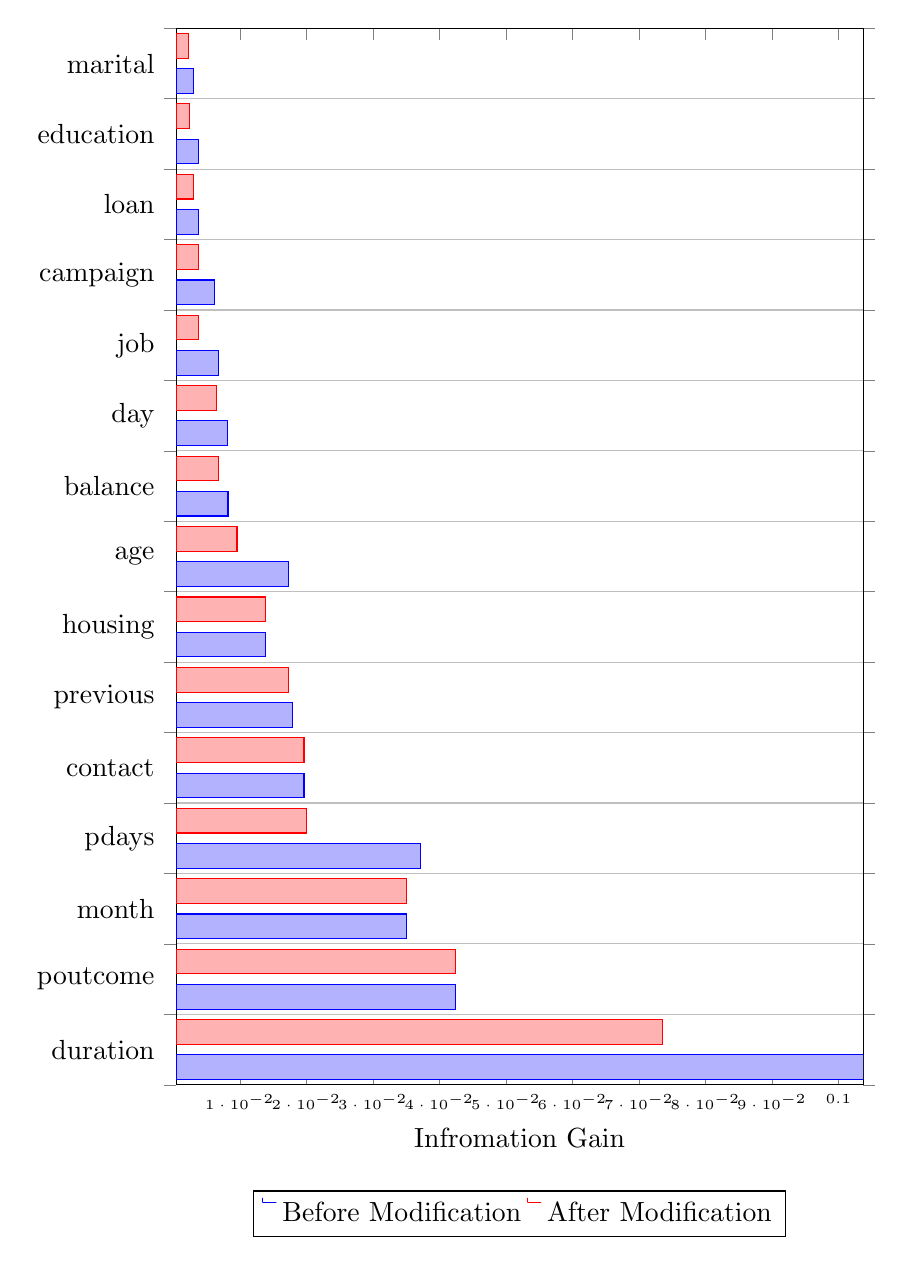
\begin{tikzpicture}
\centering
\begin{axis}[ y tick label style={/pgf/number format/1000 sep=},
	xlabel=Infromation Gain,
	enlargelimits=false,
	legend style={at={(0.5,-0.1)},
	anchor=north,legend columns=-1},
		xbar interval=0.7 ,
	x tick label style={font=\tiny},
	width=.85\textwidth,
        height=15cm,
	,yticklabels={duration, poutcome, month, pdays, contact, previous, housing, age, balance, day, job, campaign, loan, education, marital, default}
]
\addplot 
	coordinates {(0.103716,0)
(0.042411,1)
(0.035131,2)
(0.037174,3)
(0.019659,4)
(0.017869,5)
(0.013928,6)
(0.01734,7)
(0.008225,8)
(0.008119,9)
(0.0068,10)
(0.006151,11)
(0.003795,12)
(0.003748,13)
(0.003031,14)
(0.000424,15)};
\addplot 
	coordinates {
(0.073545,0)
(0.042411,1)
(0.035131,2)
(0.020041,3)
(0.019659,4)
(0.017385,5)
(0.013928,6)
(0.009584,7)
(0.0068,8)
(0.006454,9)
(0.003795,10)
(0.003748,11)
(0.003031,12)
(0.002401,13)
(0.002312,14)
(0.000424,15)};
\legend{Before Modification, After Modification}
\end{axis}
\end{tikzpicture}
\caption{Information Gain Unbalanced Dataset }
\label{fig:Information_Gain_Unbalanced_Dataset }
\end{figure}

%%%%%%%%%%%%%%  end    GRAPH1    %%%%%%%%%%%%%%%%

 \par


\section{Balanced Datasets}
The result of the balanced dataset is quite similar to the unbalanced one that J48 is the best (see \textit{Table} 5.4). However, all balanced dataset accuracies are lower than the unbalance dataset's result. The attribute ranking of this dataset defines a slightly different from the original dataset.  The top 10 attributes are 'duration', 'month', 'poutcome', 'pdays', 'contact', 'previous', 'age', 'housing', 'job', and 'balance'. 'days' attribute, which includes in the top 10 essential attributes, does not rank in this dataset.\par


%%%%%%%%%%%%%%%%%%%% Table No: 13 starts here %%%%%%%%%%%%%%%%%%%%

\begin{table}[htbp]
\centering
\begin{tabular}{|c|c|c|c|}
\hline
\multirow{2}{*}{Algorithms} & \multicolumn{3}{c|}{Accuracy} \\ \cline{2-4} 
 & 17 Attributes & 10 Attributes & 5 Attributes \\ \hline \hline
Zero Base & 52.62\% & 52.62\% & 52.62\% \\ \hline
Rules.J48 & 84.99\% & 83.44\% & 81.99\% \\ \hline
Bayes. Naive Bayes & 77.47\% & 76.31\% & 75.97\% \\ \hline
Function. Logistic Regression & 82.56\% & 82.11\% & 81.05\% \\ \hline
Lazy.IB1 & 71.46\% & 77.00\% & 77.84\% \\ \hline
\end{tabular}\caption{Balanced Dataset Result}
\label{tab:Balanced Dataset Result}
 \end{table}
%%%%%%%%%%%%%%%%%%%% Table No: 13 ends here %%%%%%%%%%%%%%%%%%%%

\par

The accuracy rate of version appears the best for both 17 and 10 attributes (see \textit{Table} 5.5). When only 5 attributes included in the dataset, version 4, 6, and 8 have a better accuracy ratio than the rest. The average outcome shows version 2 is the best.\par

%%%%%%%%%%%%%%%%%%%% Table No: 14 starts here %%%%%%%%%%%%%%%%%%%%
\begin{table}[htbp]
\centering
\begin{tabular}{|c|c|c|c|c|}
\hline
\multirow{2}{*}{Modification} & \multicolumn{4}{c|}{Accuracy} \\ \cline{2-5} 
 & 17 Attributes & 10 Attributes & 5 Attributes & Average \\ \hline \hline
Original & 84.99\% & 83.44\% & 81.99\% & 83.48\% \\ \hline
Version 1 & 84.78\% & 84.90\% & 81.99\% & 83.89\% \\ \hline
Version 2 & 85.36\% & 85.16\% & 82.12\% & 84.21\% \\ \hline
Version 3 & 84.87\% & 83.44\% & 82.12\% & 83.48\% \\ \hline
Version 4 & 84.81\% & 83.81\% & 82.62\% & 83.75\% \\ \hline
Version 5 & 84.77\% & 83.48\% & 82.12\% & 83.46\% \\ \hline
Version 6 & 84.72\% & 83.82\% & 82.62\% & 83.72\% \\ \hline
Version 7 & 84.49\% & 83.59\% & 82.12\% & 83.40\% \\ \hline
Version 8 & 84.79\% & 83.63\% & 82.62\% & 83.68\% \\ \hline
\end{tabular}\caption{Result 8 Modification Features Unbalanced Dataset}
\label{tab:Result 8 Modification Features Unbalanced Dataset}
 \end{table}
%%%%%%%%%%%%%%%%%%%% Table No: 14 ends here %%%%%%%%%%%%%%%%%%%%

\par

The result of attribute selection shows that 'duration', 'month', 'poutcome', 'pdays', and 'contact' are constantly at the top 5. As expected, the balanced dataset with an equal distribution have higher information gain values compared to the unbalanced dataset (see \textit{Figure} 5.6).\par

%%%%%%%%%%%%%%%%%%%% Table No: 15 starts here %%%%%%%%%%%%%%%%%%%%
\begin{table}[htbp]
\centering
\scalebox{0.75}{
\begin{tabular}{|c|c|c|c|c|c|c|c|c|}
\hline
Rank & Version 1 & Version 2 & Version 3 & Version 4 & Version5 & Version6 & Version 7 & Version8 \\ \hline
\multirow{16}{*}{\begin{tabular}[c]{@{}c@{}}High\\ to low\end{tabular}} & duration & duration & duration* & duration* & duration* & duration* & duration & duration* \\ \cline{2-9} 
 & month & month & month & month & month & month & month & month \\ \cline{2-9} 
 & poutcome & poutcome & poutcome & poutcome & poutcome & poutcome & poutcome & poutcome \\ \cline{2-9} 
 & pdays & contact & contact & contact & contact & contact & contact & contact \\ \cline{2-9} 
 & contact & pdays* & pdays* & pdays* & pdays* & pdays* & pdays* & pdays* \\ \cline{2-9} 
 & previous & previous* & previous* & previous & previous & previous & previous* & previous* \\ \cline{2-9} 
 & housing & age & age & age & age & age & housing & housing \\ \cline{2-9} 
 & balance & housing & housing & housing & housing & housing & age* & age* \\ \cline{2-9} 
 & day & job & job & job & job & job & job & job \\ \cline{2-9} 
 & age* & campaign & campaign & balance* & balance* & campaign & campaign & balance* \\ \cline{2-9} 
 & job & balance* & balance* & loan & loan & balance* & balance* & loan \\ \cline{2-9} 
 & campaign & loan & loan & education & education & loan & loan & education \\ \cline{2-9} 
 & loan & education & education & marital & marital & education & education & marital \\ \cline{2-9} 
 & education & marital & marital & campaign* & campaign* & marital & marital & campaign* \\ \cline{2-9} 
 & marital & day* & day* & day* & day* & day* & day* & day* \\ \cline{2-9} 
 & default & default & default & default & default & default & default & default \\ \hline
\end{tabular}
}
\caption{Balanced Dataset Attributes Rank}
\label{tab:Balanced Dataset Attributes Rank}
\raggedright
{\fontsize{8pt}{9.6pt}\selectfont \textit{$\ast$ modification feature}\par}\par
 \end{table}
%%%%%%%%%%%%%%%%%%%% Table No: 15 ends here %%%%%%%%%%%%%%%%%%%%

\par

Overall, the result shows that the unbalanced dataset gives a better result compare to the balanced dataset. The sampling method coded to produce the balanced dataset might lose some important information. For instance, the 'balance' attribute has different data range with the original or unbalanced dataset. The sampling data may less accurate to represent the whole dataset.  The highest accuracy rate with minimum feature is the unbalanced dataset version 7. Additional test changing some parameters was performed (see \textit{Table} 5.7), but the result did not improve the accuracy value. \par


%%%%%%%%%%%%%%%%%%%% Table No: 16 starts here %%%%%%%%%%%%%%%%%%%%
\begin{table}[h!]
\centering
\begin{tabular}{|c|c|}
\hline
Parameter & Accuracy \\ \hline \hline
Batch = 10; Unplace= true; Seed = 10; collapse tree = True & 90.23\% \\ \hline
Binary Split = False & 90.19\% \\ \hline
Cross Validation=8 & 90.22\% \\ \hline
Cross Validation=20 & 90.23\% \\ \hline
 \end{tabular}\caption{Version 2 Additional Parameter Test}
\label{tab:Version 2 Additional Parameter Test}
 \end{table}
%%%%%%%%%%%%%%%%%%%% Table No: 16 ends here %%%%%%%%%%%%%%%%%%%%
\par

%%%%%%%%%%%%%%     GRAPH2    %%%%%%%%%%%%%%%%
\begin{figure}[htbp]
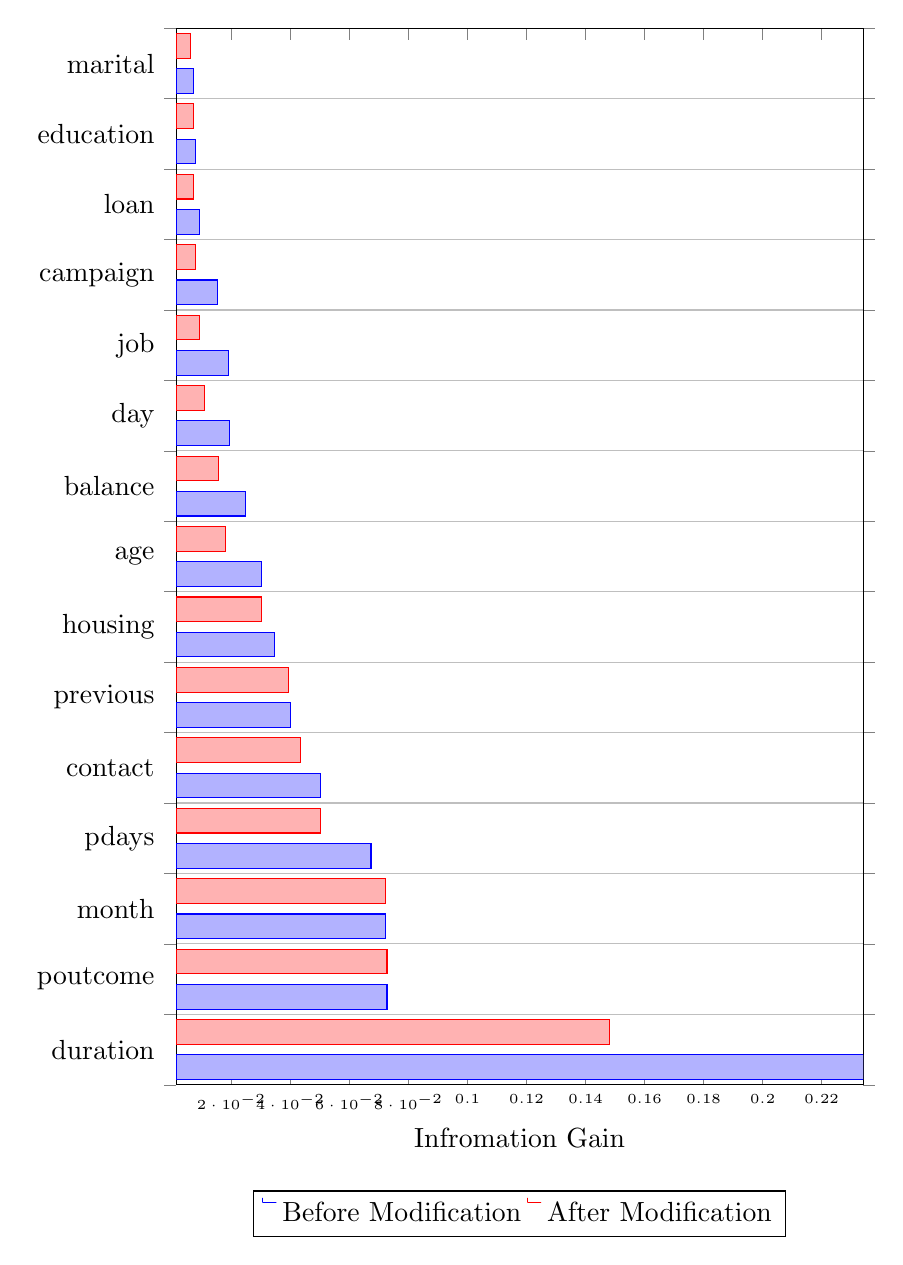
\begin{tikzpicture}
\centering
\begin{axis}[ y tick label style={/pgf/number format/1000 sep=},
	xlabel=Infromation Gain,
	enlargelimits=false,
	legend style={at={(0.5,-0.1)},
	anchor=north,legend columns=-1},
		xbar interval=0.7 ,
	x tick label style={font=\tiny},
	width=.85\textwidth,
        height=15cm,
	,yticklabels={duration, poutcome, month, pdays, contact, previous, housing, age, balance, day, job, campaign, loan, education, marital, default}
]
\addplot 
	coordinates {(0.23407,0)
(0.07269,1)
(0.0723,2)
(0.06728,3)
(0.05009,4)
(0.03985,5)
(0.03472,6)
(0.03023,7)
(0.02488,8)
(0.01923,9)
(0.01912,10)
(0.01521,11)
(0.00901,12)
(0.00795,13)
(0.00708,14)
(0.00123,15)};
\addplot 
	coordinates {
(0.14816,0)
(0.07269,1)
(0.0723,2)
(0.05009,3)
(0.04326,4)
(0.03933,5)
(0.03023,6)
(0.01805,7)
(0.01558,8)
(0.01083,9)
(0.00901,10)
(0.00795,11)
(0.00708,12)
(0.00701,13)
(0.0061,14)
(0.00123,15)};
\legend{Before Modification, After Modification}
\end{axis}
\end{tikzpicture}
\caption{Information Gain Balanced Dataset }
\label{fig:Information_Gain_Balanced_Dataset }
\end{figure}

%%%%%%%%%%%%%%  end    GRAPH2    %%%%%%%%%%%%%%%%







\chapter{Bank Marketing Prediction System Prototype}
\section{Back-end}
The back-end programming language used for developing a prototype of  bank marketing prediction system was Python 2.7 under the Anaconda1 platform on macOS High Sierra version 10.13.4. with 1.1 GHz Intel Core M processor. An integration development tool, PyCharm Community Edition tool largely supported the development. The unbalanced dataset combination 7 with five attributes, which shows the best result from WEKA experiment, was stored in CSV format.  There are some libraries used such as sklearn, numpy, panda, cgi, etc. Python-WEKA-wrapper API runs the J48 classifier, and then calculates the accuracy rate as well as saves tree prune information in JSON format.  The prediction system evaluates the new added client information based on the stored previous dataset. This application can be accessed locally, using CGIHTTPServer, and can work on multiple platforms, using Ngrok, a reverse proxy software to establish secure tunnels(see \textit{Figure} 6.1) .\par

\begin{figure}[htbp]
\centering
		\includegraphics[scale=0.5]{/Users/imeiliasantoso/Desktop/latexfile/master_project/example-simple/media/image1.png}
		\caption{Back-end flow}
		\label{fig:Backend_flow}
	
\end{figure}


\section{Front-end}


The front-end was coded using JavaScript, HTML, and CSS. There are three pages at the front end such as visualization, registration, and prediction pages.  The visualization page helps bank marketers to understand their customers' tendency so that they can make a better decision effectively. Amcharts and D3 library was implemented to display interactive graphs and charts. Since a bar chart is best used to compare different value and to present distribution clearly \cite{Mat151}, the attributes was predominantly displayed in column and histogram charts (see \textit{Figure} 6.3). The registration page allows bank marketer to add new training data and then recalculate a new accuracy rate (see \textit{Appendix} C \textit{Figure} 7.5). This page can help bank marketer to understand if a new registered client data can improve the accuracy or not. If the accuracy decreases, the client might not match the tendency of the majority group. Therefore, bank marketers can learn the client behavior, profile, and other factors that may influence the outcome. Bank marketer are also able to predict the potential client result at prediction page (see \textit{Appendix} D \textit{Figure} 7.6). The function of this page is to forecast whether the clients will likely to subscribe the campaign or not based on their profile information such as age, occupation, marital status, education background, and contact method, and based on previous campaign data, such as how long the phone calls done during previous or current campaign, when they were contacted, how many days passed by after they were last contacted, how many times they were calls, and the result of previous campaign. Since previous campaign data combination was selected from WEKA experiment, the prediction based on this combination give a higher accuracy result compared to accuracy from the client profile. Decision Tree that can help bank marketer to understand how the J48 algorithm works is also displayed at prediction page using previous campaign data (see \textit{Appendix} D \textit{Figure} 7.7).\par

\begin{figure}[htbp]
\centering
		\includegraphics[scale=0.5]{/Users/imeiliasantoso/Desktop/latexfile/master_project/example-simple/media/image2.png}
		\caption{Application Back-end and Front-end Flow}
		\label{fig:Application_Backend_and_Frontend_Flow}
	
\end{figure}

\begin{figure}[htbp]
\centering
		\includegraphics[scale=0.35]{/Users/imeiliasantoso/Desktop/latexfile/master_project/example-simple/media/image3.png}
		\caption{Visualization Page}
		\label{fig:Visualization_Page}
	
\end{figure}



\section{Prediction Cases Based on Previous Campaign}

In total, there are 88 leaves and 133 trees (see \textit{Figure} 6.4). One of the shortest case example needs only two parameters to make a prediction. For instance, if the phone duration is less than 440 seconds and the previous result is failure, the client will likely not to subscribe the current or future campaign. On the other hand, if the duration is more than 132 seconds and previous campaign result is success, this type of client might subscribe the campaign. Some cases need four parameters to find out the result.  If the phone duration is more than 647 seconds, previous outcome is failure, phone call is done in February, and days passed by after last contact is between 365 and 720 days, there are the opportunity this client will subscribe the campaign.\par

\begin{figure}[h!]
\centering
		\includegraphics[scale=0.25]{/Users/imeiliasantoso/Desktop/latexfile/master_project/example-simple/media/image4.png}
\caption{Full Decision Tree}
	
\end{figure}


\chapter{Conclusion and Future Work}
This research project has projected minimum attributes required for predicting the potential bank customers who want to subscribe to new campaigns efficiently.
The result shows that information from previous campaigns such as 'duration, 'poutcome', 'month', 'pdays' and 'previous' are the significant attributes that can help bank marketers to make decision.  
The 'pdays' attribute was modified into six groups. Generally, the modified features have increased the accuracy rate and created better cut points of decision trees.   
The original unbalanced dataset outperforms the balanced dataset, which was altered using the under-sampling method. Currently, these studies did not focus on how to create a better performance of a balanced dataset. However, it is necessary to bring up this topic in the future.
The result gives the direction for further work to validate the correlation between previous campaign including 'duration','poutcome', 'month', 'pdays', 'day', 'previous', 'campaign' and customer information 'age', 'balance', 'job', 'campaign', 'loan', 'education', and 'marital' to determine the minimum customer attribute information to make decision.\par


\bibliographystyle{plain}
\bibliography{simple}
 %\backrefpagesname
 \nocite{*}
\newpage




\section*{Appendices}
\subsection*{Appendix A: Outliers of Unbalanced Dataset and Balanced Dataset}
\addcontentsline{toc}{subsection}{Appendix A: Outliers of Unbalanced Dataset and Balanced Dataset}
\par
\begin{figure}[h]
\centering
		\includegraphics[width=12cm]{/Users/imeiliasantoso/Desktop/latexfile/master_project/example-simple/media/image5.png}
		\caption{Unbalanced Dataset Outliers}
		\label{fig:Unbalanced_Dataset_Outliers}	
\end{figure}
\par

\begin{figure}[h!]
\centering
	\includegraphics[width=12cm]{/Users/imeiliasantoso/Desktop/latexfile/master_project/example-simple/media/image6.png}
		\caption{Balanced Dataset Outliers}
		\label{fig:Balanced_Dataset_Outliers}
\end{figure}

\clearpage
\newpage

\subsection*{Appendix B: Attributes Displayed on Visualization Page}
\addcontentsline{toc}{subsection}{Appendix B: Attributes Displayed on Visualization Page}

\begin{figure}[h]
\centering
	\includegraphics[width=12cm]{/Users/imeiliasantoso/Desktop/latexfile/master_project/example-simple/media/image7.png}
	\caption{Job Attribute and Marital Attribute}
		\label{fig:Job_Attribute_and_Marital_Attribute}
\end{figure}

\begin{figure}[h!]
\centering
	\includegraphics[width=12cm]{/Users/imeiliasantoso/Desktop/latexfile/master_project/example-simple/media/image8.png}
		\caption{All Attributes' Class}
		\label{fig:All_Attributes_Class}
\end{figure}
\par


\clearpage
\newpage


\subsection*{Appendix C: Registration Page}
\addcontentsline{toc}{subsection}{Appendix C: Registration Page}
\begin{figure}[htbp]
\centering
	\includegraphics[width=15cm]{/Users/imeiliasantoso/Desktop/latexfile/master_project/example-simple/media/image9.png}
			\caption{Registration Page}
		\label{fig:Registration_Page}
\end{figure}

\clearpage
\newpage



\subsection*{Appendix D: Prediction Page}
\addcontentsline{toc}{subsection}{Appendix D: Prediction Page}
\begin{figure}[htbp]
\centering
	\includegraphics[width=15cm]{/Users/imeiliasantoso/Desktop/latexfile/master_project/example-simple/media/image10.png}
\caption{Prediction Page Based on Previous Campaign}
		\label{fig:Prediction_Page_Based_on_Previous_Campaign}
\end{figure}


\begin{figure}[h!]
\centering
	\includegraphics[width=15cm]{/Users/imeiliasantoso/Desktop/latexfile/master_project/example-simple/media/image11.png}
\caption{Decision Tree}
		\label{fig:Decision_Tree}
\end{figure}

\clearpage
\newpage

\subsection*{Appendix E: Register Page Back-End Source Code}
\addcontentsline{toc}{subsection}{Appendix D: Register Page Back-End Source Code}

\begin{lstlisting}[language=Python]

import weka.core.jvm as jvm
from weka.core.converters import Loader, Saver
from weka.classifiers import Classifier
from weka.classifiers import Evaluation
from weka.core.classes import Random
import weka.plot.graph as plot_graph
import re
import numpy as np
import string
import HTMLParser
import nltk
from nltk.stem.porter import PorterStemmer
import cgi, cgitb
import json
import sys, os
import pandas as pd
import csv as csv
from pre2_register import run

cgitb.enable()
form = cgi.FieldStorage()

name = eval(form.getvalue('name'))
age = eval(form.getvalue('age'))
duration = eval(form.getvalue('duration'))
day = eval(form.getvalue('day'))
month = eval(form.getvalue('month'))
balance = eval(form.getvalue('balance'))
campaign = eval(form.getvalue('campaign'))
pdays = eval(form.getvalue('pdays'))
previous = eval(form.getvalue('previous'))
radio1_job = eval(form.getvalue('radio1_job'))
radio2_job = eval(form.getvalue('radio2_job'))
radio3_job = eval(form.getvalue('radio3_job'))
radio1_status = eval(form.getvalue('radio1_status'))
radio2_status = eval(form.getvalue('radio2_status'))
radio3_status = eval(form.getvalue('radio3_status'))
radio1_edu = eval(form.getvalue('radio1_edu'))
radio2_edu = eval(form.getvalue('radio2_edu'))
radio3_edu = eval(form.getvalue('radio3_edu'))
radio4_edu = eval(form.getvalue('radio4_edu'))
radio1_contact = eval(form.getvalue('radio1_contact'))
radio2_contact = eval(form.getvalue('radio2_contact'))
radio3_contact = eval(form.getvalue('radio3_contact'))
radio1_hs = eval(form.getvalue('radio1_hs'))
radio2_hs = eval(form.getvalue('radio2_hs'))
radio1_loan = eval(form.getvalue('radio1_loan'))
radio2_loan = eval(form.getvalue('radio2_loan'))
radio1_def = eval(form.getvalue('radio1_def'))
radio2_def = eval(form.getvalue('radio2_def'))
radio1_pout = eval(form.getvalue('radio1_pout'))
radio2_pout = eval(form.getvalue('radio2_pout'))
radio3_pout = eval(form.getvalue('radio3_pout'))
radio4_pout = eval(form.getvalue('radio4_pout'))
radio1_y = eval(form.getvalue('radio1_y'))
radio2_y = eval(form.getvalue('radio2_y'))
radio3_y = eval(form.getvalue('radio3_y'))

data = pd.read_csv('/../bank-full_input.csv')
l = len(data) + 1

age = str(age)
duration = str(duration)
month = str(month)
campaign = str(campaign)
balance = str(balance)
day = str(day)
pdays = str(pdays)
previous = str(previous)

job = ""
marital = ""
education = ""
default = ""

housing = ""
loan = ""

poutcome =""
y =""

#job
if (radio1_job == 'Emplyoed'):
	job = "emplyoed"

if (radio2_job == 'Unemplyoed'):
	job = "unemplyoed"

if (radio2_job == 'Unknown'):
	job = "unknown"

#status
if (radio1_status == 'Married'):
	marital = "married"

if (radio2_status== 'Unmarried'):
	marital = "unmarried"

if (radio3_status == 'Unknown'):
	marital = "unknown"

#edu
if (radio1_edu == 'Primary'):
	education = "primary"

if (radio2_edu == 'Secondary'):
	education = "secondary"

if (radio3_edu == 'Teritory'):
	education = "teritory"

if (radio4_edu == 'Unknown'):
	education = "unknown"

 #Contact
if (radio1_contact == 'Telephone'):
	contact = "telephone"

if (radio2_contact == 'Cellular'):
	contact = "cellular"

if (radio3_contact == 'Unknown'):
	contact = "unknown"

#poutcome
if (radio1_pout == 'Success'):
	poutcome = "success"

if (radio2_pout == 'Failure'):
	poutcome = "failure"

if (radio3_pout == 'Other'):
	poutcome = "other"

if (radio4_pout == 'Unknown'):
	poutcome = "unknown"

#result
if (radio1_y == 'Yes'):
	y = "yes"

if (radio2_y == 'No'):
	y = "no"

df = pd.DataFrame(data)

df1 = pd.DataFrame({'age':[age],
		'job':[job],
		'marital':[marital],
		'education':[education],
		'contact':[contact],
		'balance':[balance],
		'housing':[housing],
		'loan':[loan],
		'default':[default],
		'duration':[duration],
		'day':[day],
		'month':[month],
		'campaign':[campaign],
		'pdays':[pdays],
		'previous':[previous],
		'poutcome':[poutcome],
		'y':[y]})

df2 = df.append(df1)
df2.to_csv('..../bank-full_input.csv', index = False)

accuracy = run()
Result_Accuracy = accuracy

print "Content-type:application/json\r\n\r\n"
print json.dumps({'status':'yes',
	'Result_Accuracy':json.dumps(Result_Accuracy)})
print ""
run()

#call run()
def run():
    jvm.start()
    load_csv = Loader("weka.core.converters.CSVLoader")
    data_csv = load_csv.load_file(
        "/../bank-full_input.csv")

    saver = Saver("weka.core.converters.ArffSaver")
    saver.save_file(data_csv,
                    "/../bank-full_input.arff")

    load_arff = Loader("weka.core.converters.ArffLoader")
    data_arff = load_arff.load_file(
       		"/../bank-full_input.arff")
    data_arff.class_is_last()

    cls = Classifier(classname="weka.classifiers.trees.J48")
    cls.build_classifier(data_arff)
    for index, inst in enumerate(data_arff):
        pred = cls.classify_instance(inst)
        dist = cls.distribution_for_instance(inst)
        # save tree prune in txt file

    saveFile = open("/../bank-full_input.txt", "w")
    saveFile.write(str(cls))
    # print(cls)
    saveFile.close()

    global j48
    J48_class = Classifier(classname="weka.classifiers.trees.J48",
    		options=["-C", "0.25", "-M", "2"])
    
    J48_class.build_classifier(data_arff)
    evaluationj48 = Evaluation(data_arff)
    
    evaluationj48.crossvalidate_model(J48_class, 
    		data_arff , 10, Random(100))
    j48 = str(evaluationj48.percent_correct)
    jvm.stop()
    return j48
\end{lstlisting}



\clearpage
\newpage

\subsection*{Appendix F: Register Page Front-End Source Code}
\addcontentsline{toc}{subsection}{Appendix F: Register Page Front-End Source Code}
\begin{lstlisting}[language=HTML]
<!DOCTYPE HTML>
<html>
<head>
<title>Bank Marketing Dataset</title>
<meta http-equiv="Content-Type" content="text/html; charset=utf-8" />
	....
	....
	....
	
  <div>
    <div class="pageCont">
    <div class="wrap">
<header class="pageCont_header">
  <h1>New Client Data</h1>
  <p>Add New the Trainnning Data</p>
</header>

<section class="pageCont_main">
<h2>User Profile </h2>
<p class="formTitle">Name : </p>
<input id="name" type="text"
	 name="name" value="Imeila Santoso"><br> <br>
<p class="formTitle">Age  : </p>
<input id="age" type="text" 
	name="age" value="29" ><br> <br>

<form name="form1">
<p class="formTitle">Job :</p>
  <label><input id="Radio1" type="radio" 
  	name="Radio1" checked="checked">Emplyoed</label>
  <label><input id="Radio2" type="radio" 
  	name="Radio1">Unemplyoed</label>
  <label><input id="Radio3" type="radio" 
  	name="Radio1">Unknown</label><br><br>
</form>

<form name="form2">
<p class="formTitle">Marital :</p>
  <label><input id="Radio1" type="radio" 
  	name="Radio1" checked="checked">Married</label>
  <label><input id="Radio2" type="radio" 
  	name="Radio1">Unmarried</label>
  <label><input id="Radio3" type="radio" 
  	name="Radio1">Unknown</label><br><br>
</form>

<form name="form3">
<p class="formTitle">Education :</p>
  <label><input id="Radio1" type="radio" 
  	name="Radio1" checked="checked">Primary</label>
  <label><input id="Radio2" type="radio" 
  	name="Radio1">Secondary</label>
  <label><input id="Radio3" type="radio" 
  	name="Radio1">Teritory</label>
  <label><input id="Radio4" type="radio" 
  	name="Radio1">Unknown</label><br><br>
</form>

<form name="form4">
<p class="formTitle">Contact:</p>
  <label><input id="Radio1" type="radio" 
  	name="Radio1" checked="checked">Telephone</label>
  <label><input id="Radio2" type="radio" 
  	name="Radio1">Cellular</label>
  <label><input id="Radio2" type="radio" 
  	name="Radio1">Unknown</label><br><br>
</form>

<p class="formTitle">Balance: </p>
<input id="balance" type="text" name="balace" value="300" >
in Euro <br> <br>
 
<form name="form6">
<p class="formTitle">Housing:</p>
  <label><input id="Radio1" type="radio" 
  	name="Radio1" checked="checked">Yes</label>
  <label><input id="Radio2" type="radio" 
  	name="Radio1">No</label><br><br>
</form>

<form name="form7">
<p class="formTitle">Loan:</p>
  <label><input id="Radio1" type="radio" 
  	name="Radio1" checked="checked">Yes</label>
  <label><input id="Radio2" type="radio"
  	name="Radio1">No</label><br><br>
</form>

<form name="form8">
<p class="formTitle">Deafult:</p>
  <label><input id="Radio1" type="radio" 
  	name="Radio1" checked="checked">Yes</label>
  <label><input id="Radio2" type="radio" 
  	name="Radio1">No</label><br><br>
</form>

<h2>Previous Campaign Result</h2>

<p class="formTitle">Duration  : 
</p><input id="duration" type="text" 
	name="duration" value="30" ><br><br>
<p class="formTitle">Day : 
</p><input id="day" type="text" 
	name="day" value="1"><br><br>
<p class="formTitle">Month  : 
</p><input id="month" type="text" 
	name="month" value="mar"><br><br>
<p class="formTitle">Campaign  : 
</p><input id="campaign" type="text" 
	name="campaign" value="10" ><br><br>
<p class="formTitle">Previous Days  : 
</p><input id="pdays" type="text" 
	name="pdays" value="10" ><br>
<p class="formTitle">Previous Contacts  : 
</p><input id="previous" type="text" 
	name="previous" value="10" ><br>


<form name="form12">
<p class="formTitle">Previous Outcome:</p>
  <label><input id="Radio1" type="radio" 
  	name="Radio1" checked="checked">Sucess</label>
  <label><input id="Radio2" type="radio" 
  	name="Radio1">Failure</label>
  <label><input id="Radio3" type="radio" 
  	name="Radio1">Other</label>
  <label><input id="Radio4" type="radio" 
  	name="Radio1">Unknown</label><br><br>
</form>

<h2>Current Result</h2>
<form name="form13">
<p class="formTitle">Result:</p>
  <label><input id="Radio1" type="radio" 
  	name="Radio1" checked="checked">Yes</label>
  <label><input id="Radio2" type="radio" 
  	name="Radio1">No</label>
  <label><input id="Radio3" type="radio" 
  	name="Radio1">Unknown</label><br><br>
</form>


<button onclick="sendData()">
  Register
</button>

</section> </div> </div>


<script>
function sendData(){

var name = document.getElementById("name").value
var age = document.getElementById("age").value
var duration = document.getElementById("duration").value
var balance = document.getElementById("balance").value
var day = document.getElementById("day").value
var month = document.getElementById("month").value
var campaign = document.getElementById("campaign").value
var pdays = document.getElementById("pdays").value
var previous = document.getElementById("previous").value

// Job
if (document.form1.Radio1[0].checked) {
  radio1_job = "Emplyoed";
  radio2_job = "False";
  radio3_job = "False";
} else {
  radio1_job = "False";
}

if (document.form1.Radio1[1].checked) {
  radio2_job = "Unemplyoed";
  radio3_job = "False" 
  radio1_job = "False"
} else {
  radio2_job = "False";
}


if (document.form1.Radio1[2].checked) {
  radio3_job = "Unknown";
  radio1_job = "False";
  radio2_job = "False" 
} else {
  radio3_job = "False";
}

////////////////// // radio for status
if (document.form2.Radio1[0].checked) {
  radio1_status = "Married";
  radio2_status = "False";
  radio3_status = "False";
} else {
  radio1_status = "False";
}

if (document.form2.Radio1[1].checked) {
  radio2_status = "Unmarried";
  radio3_status = "False" 
  radio1_status = "False"
} else {
  radio2_status = "False";
}

if (document.form2.Radio1[2].checked) {
  radio3_status = "Unknown";
  radio1_status = "False";
  radio2_status = "False" 
} else {
  radio3_status = "False";
}

////////////////// // radio for education
if (document.form3.Radio1[0].checked) {
  radio1_edu = "Primary";
  radio2_edu = "False";
  radio3_edu = "False";
  radio4_edu = "False";
} else {
  radio1_edu = "False";
}

if (document.form3.Radio1[1].checked) {
  radio2_edu = "Secondary";
  radio3_edu = "False"
  radio4_edu = "False";
  radio1_edu = "False"
} else {
  radio2_status = "False";
}


if (document.form3.Radio1[2].checked) {
  radio3_edu = "Teritory";
  radio4_edu = "False";
  radio1_edu = "False";
  radio2_edu = "False" 
} else {
  radio3_edu = "False";
}

if (document.form3.Radio1[3].checked) {
  radio4_edu = "Unknown";
  radio1_edu = "False";
  radio3_edu = "False";
  radio2_edu = "False"
} else {
  radio4_edu = "False";
}



// radio for contact
if (document.form4.Radio1[0].checked) {
  radio1_contact = "Telephone";
  radio2_contact = "False";
  radio3_contact = "False";
} else {
  radio1_contact = "False";
}

if (document.form4.Radio1[1].checked) {
  radio2_contact = "Cellular";
  radio3_contact = "False" 
  radio1_contact = "False"
} else {
  radio2_contact = "False";
}

if (document.form4.Radio1[2].checked) {
  radio3_contact = "Unknown";
  radio1_contact = "False";
  radio2_contact = "False" 
} else {
  radio3_contact = "False";
}


////////////////// // radio for Housing
if (document.form6.Radio1[0].checked) {
  radio1_hs = "Yes";
  radio2_hs = "False";
} else {
  radio1_hs = "False";
}

if (document.form6.Radio1[1].checked) {
  radio2_hs = "No";
  radio1_hs = "False"
} else {
  radio2_hs = "False";
}

////////////////// // radio for Loan
if (document.form7.Radio1[0].checked) {
  radio1_loan = "Yes";
  radio2_loan = "False";
} else {
  radio1_loan = "False";
}

if (document.form7.Radio1[1].checked) {
  radio2_loan = "No";
  radio1_loan = "False"
} else {
  radio2_loan = "False";
}

////////////////// // radio for default
if (document.form8.Radio1[0].checked) {
  radio1_def = "Yes";
  radio2_def = "False";
} else {
  radio1_def = "False";
}

if (document.form8.Radio1[1].checked) {
  radio2_def = "No";
  radio1_def = "False"
} else {
  radio2_def = "False";
}

if (document.form12.Radio1[0].checked) {
  radio1_pout = "Success";
  radio2_pout = "False";
  radio3_pout = "False";
  radio4_pout = "False";
} else {
  radio1_edu = "False";
}

if (document.form12.Radio1[1].checked) {
  radio2_pout = "Failure";
  radio3_pout = "False"
  radio4_pout = "False";
  radio1_pout = "False"
} else {
  radio2_pout = "False";
}

if (document.form12.Radio1[2].checked) {
  radio3_pout = "Other";
  radio4_pout = "False";
  radio1_pout = "False";
  radio2_pout = "False" 
} else {
  radio3_pout = "False";
}

if (document.form12.Radio1[3].checked) {
  radio4_pout = "Unknown";
  radio1_pout = "False";
  radio3_pout = "False";
  radio2_pout = "False"
} else {
  radio4_pout = "False";
}

////////////////// // radio for current result
if (document.form13.Radio1[0].checked) {
  radio1_y = "Yes";
  radio2_y = "False";
  radio3_y = "False";
} else {
  radio1_y = "False";
}

if (document.form13.Radio1[1].checked) {
  radio2_y = "No";
  radio3_y = "False" 
  radio1_y = "False"
} else {
  radio2_y = "False";
}

if (document.form13.Radio1[2].checked) {
  radio3_y = "Unknown";
  radio1_y = "False";
  radio2_y = "False" 
} else {
  radio3_y = "False";
}

$.ajax({
    type: "POST",
    url: "/cgi-bin/pre1_register.py",
    data: { name:JSON.stringify(name),
    age:JSON.stringify(age),
    duration:JSON.stringify(duration),
    day:JSON.stringify(day),
    month:JSON.stringify(month),
    campaign:JSON.stringify(campaign),
    radio1_job:JSON.stringify(radio1_job),
    radio2_job:JSON.stringify(radio2_job),
    radio3_job:JSON.stringify(radio3_job),
    radio1_status:JSON.stringify(radio1_status),
    radio2_status:JSON.stringify(radio2_status),
    radio3_status:JSON.stringify(radio3_status),
    radio1_edu:JSON.stringify(radio1_edu),
    radio2_edu:JSON.stringify(radio2_edu),
    radio3_edu:JSON.stringify(radio3_edu),
    radio4_edu:JSON.stringify(radio4_edu),
    radio1_contact:JSON.stringify(radio1_contact),
    radio2_contact:JSON.stringify(radio2_contact),
    radio3_contact:JSON.stringify(radio3_contact),
    balance:JSON.stringify(balance),
    radio1_hs:JSON.stringify(radio1_hs),
    radio2_hs:JSON.stringify(radio2_hs),
    radio1_loan:JSON.stringify(radio1_loan),
    radio2_loan:JSON.stringify(radio2_loan),
    radio1_def:JSON.stringify(radio1_def),
    radio2_def:JSON.stringify(radio2_def),
    pdays:JSON.stringify(pdays),
    previous:JSON.stringify(previous),
    radio1_pout:JSON.stringify(radio1_pout),
    radio2_pout:JSON.stringify(radio2_pout),
    radio3_pout:JSON.stringify(radio3_pout),
    radio4_pout:JSON.stringify(radio4_pout),
    radio1_y:JSON.stringify(radio1_y),
    radio2_y:JSON.stringify(radio2_y),
    radio3_y:JSON.stringify(radio3_y)},
    async: true,  
    success: function( msg ) {
    
    var status = msg['status'];

    console.log("tws")
    console.log(status)

    if (status == "yes") {
      var Result_Accuracy_Original = msg['Result_Accuracy_Original'];
      document.getElementById("result").innerHTML 
      		= Result_Accuracy
      document.getElementById("result2").innerHTML 
      		= Result_Accuracy_Original

    }
    else {
      errorMessage = "result_"
      errorMessage += msg['except']
      alert(errorMessage);
    }  
    },
    error: function(msg){     
    alert("Error sending data!");
    }
  }); 
}

</script>

  </div>
 <!--footer section start-->
     ...
    ...

</body>
</html>
\end{lstlisting}

\clearpage
\newpage
\subsection*{Appendix G: Decision Tree Visualization Front-End Source Code}
\addcontentsline{toc}{subsection}{Appendix G: Decision Tree Visualization Front-End Source Code}
\begin{lstlisting}
function showTree(){

var width = 800,
    height = 550;

var cluster = d3.layout.cluster()
    .size([height, width - 160]);

var diagonal = d3.svg.diagonal()
    .projection(function(d) { return [d.y, d.x]; });

var svg = d3.select("body").append("svg")
    .attr("width", width)
    .attr("height", height)
  .append("g")
    .attr("transform", "translate(40,0)");

d3.json("/../predict2_data.json", function(error, root)  {
  var nodes = cluster.nodes(root),
      links = cluster.links(nodes);

  var link = svg.selectAll(".link")
      .data(links)
    .enter().append("path")
      .attr("class", "link")
      .attr("d", diagonal);

  var node = svg.selectAll(".node")
      .data(nodes)
    .enter().append("g")
      .attr("class", "node")
      .attr("transform", function(d) { 
 		return "translate(" + d.y + "," + d.x + ")"; })

  node.append("circle")
      .attr("r", 4.5);

  node.append("text")
      .attr("dx", function(d) { 
      	return d.children ? -8 : 8; })
      .attr("dy", 3)
      .style("text-anchor", function(d) { 
      	return d.children ? "end" : "start"; })
      .text(function(d) { return d.name; });
});

d3.select(self.frameElement).style("height", height + "px");
}
\end{lstlisting}
\end{document}

% You may ignore or delete these two lines of comments.
% $Id: simple.tex 386 2012-11-12 15:11:16Z vlado $
